\documentclass[12pt,a4paper]{article}
\usepackage[UTF8]{ctex}
\usepackage{amsmath,amssymb}
\usepackage{listings}
\usepackage{xcolor}
\usepackage{hyperref}
\usepackage{geometry}
\usepackage{graphicx}
\geometry{margin=2.5cm}

\lstdefinestyle{python}{
  language=Python,
  basicstyle=\ttfamily\small,
  keywordstyle=\color{blue}\bfseries,
  commentstyle=\color{gray},
  stringstyle=\color{red},
  showstringspaces=false,
  breaklines=true,
  frame=single,
  backgroundcolor=\color{gray!10}
}

\title{Superdense Coding / 超密编码}
\author{QuoNic}
\date{}

\begin{document}
\maketitle

\begin{center}
\textbf{Communication / 通信} | 难度：中级 | 预计时间：10 分钟
\end{center}

\tableofcontents
\newpage

%% ============================================================
\section{为什么需要？}

超密编码使用 1 个量子比特传输 2 个经典比特，是量子通信的重要协议。

\subsection{经典局限}
\begin{itemize}
  \item 经典通信：1 个量子比特只能传输 1 个经典比特
  \item 经典通信需要 2 个信道传输 2 比特信息
\end{itemize}

\subsection{量子优势}
\begin{itemize}
  \item 超密编码：1 个量子比特传输 2 个经典比特
  \item 利用纠缠实现信息压缩
  \item 是量子通信的基础协议
\end{itemize}

\subsection{实际应用}
\begin{itemize}
  \item 量子通信（高效信息传输）
  \item 量子网络（量子互联网）
  \item 量子密码学（量子密钥分发）
\end{itemize}

%% ============================================================
\section{快速上手}

\begin{lstlisting}[style=python]
from quonic.algorithms import superdense_coding

# Send 2 classical bits using 1 qubit
result = superdense_coding("10")
print(f"Sent: {result.sent}")
print(f"Received: {result.received}")
\end{lstlisting}

\textbf{预期输出}：
\begin{verbatim}
Sent: 10
Received: 10
\end{verbatim}

%% ============================================================
\section{原理详解}

\subsection{电路图}

\begin{center}
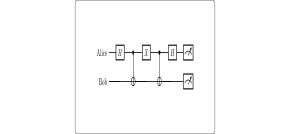
\includegraphics[width=0.6\textwidth]{../../images/superdense_coding_circuit.svg}
\end{center}

\subsection{数学推导}

超密编码协议：
\begin{enumerate}
  \item Alice 和 Bob 共享 Bell 对 $|\Phi^+\rangle = (|00\rangle + |11\rangle)/\sqrt{2}$
  \item Alice 根据要发送的 2 比特信息编码：
  \begin{itemize}
    \item 00: 不操作
    \item 01: 施加 $X$ 门
    \item 10: 施加 $Z$ 门
    \item 11: 施加 $ZX$ 门
  \end{itemize}
  \item Alice 发送她的量子比特给 Bob
  \item Bob 解码得到 2 比特信息
\end{enumerate}

\subsection{几何解释}

超密编码利用纠缠作为量子信道。Alice 的操作改变了 Bell 对的纠缠结构，Bob 通过解码恢复信息。

%% ============================================================
\section{代码详解}

\begin{lstlisting}[style=python]
from quonic.algorithms import superdense_coding

# superdense_coding(message)
# message: 2-bit string to send
result = superdense_coding("10")

# result.sent: original message
# result.received: decoded message
print(f"Sent: {result.sent}")
print(f"Received: {result.received}")
\end{lstlisting}

%% ============================================================
\section{进阶用法}

\subsection{场景 1：不同消息}

\begin{lstlisting}[style=python]
# Send different messages
for msg in ["00", "01", "10", "11"]:
    result = superdense_coding(msg)
    print(f"Sent: {msg}, Received: {result.received}")
\end{lstlisting}

\subsection{场景 2：带噪声的超密编码}

\begin{lstlisting}[style=python]
# Superdense coding with noise
result = superdense_coding("10", noise=0.05)
print(f"Error rate: {result.error_rate}")
\end{lstlisting}

%% ============================================================
\section{适用场景}

\subsection{量子通信}

超密编码可以提高量子通信的效率。

\subsection{量子网络}

超密编码是量子网络的基础协议之一。

\subsection{量子密码学}

超密编码可以用于量子密钥分发。

%% ============================================================
\section{常见问题}

\subsection{超密编码为什么能传输 2 比特？}

超密编码利用纠缠作为量子信道。Alice 的操作改变了 Bell 对的纠缠结构，Bob 通过解码恢复 2 比特信息。

\subsection{超密编码和隐形传态有什么区别？}

超密编码：1 个量子比特传输 2 个经典比特。隐形传态：2 个经典比特传输 1 个量子比特。

\subsection{超密编码需要多少量子比特？}

超密编码需要 2 个量子比特：1 个 Alice 的，1 个 Bob 的（共享 Bell 对）。

%% ============================================================
\section{学习路径}

\subsection{前置知识}
\begin{itemize}
  \item Bell 态（2 量子比特纠缠）
  \item CNOT 门和 Hadamard 门
  \item 量子测量
\end{itemize}

\subsection{继续学习}
\begin{itemize}
  \item 量子隐形传态
  \item 量子密钥分发
  \item 量子网络
\end{itemize}

%% ============================================================
\section{完整示例代码}

\subsection{示例 1：基本超密编码}

\begin{lstlisting}[style=python]
from quonic.algorithms import superdense_coding

result = superdense_coding("10")
print(f"Sent: {result.sent}")
print(f"Received: {result.received}")
\end{lstlisting}

\end{document}
